%%%%%%%%%%%%%%%%%%%%%%%%%%%%%%%%%%%%%%%%%
% Beamer Presentation
% LaTeX Template
% Version 1.0 (10/11/12)
%
% This template has been downloaded from:
% http://www.LaTeXTemplates.com
%
% License:
% CC BY-NC-SA 3.0 (http://creativecommons.org/licenses/by-nc-sa/3.0/)
%
%%%%%%%%%%%%%%%%%%%%%%%%%%%%%%%%%%%%%%%%%

%----------------------------------------------------------------------------------------
%	PACKAGES AND THEMES
%----------------------------------------------------------------------------------------
\PassOptionsToPackage{subsection=false}{beamerouterthememiniframes}
\documentclass{beamer}
\usepackage{listings}
\usepackage{mdframed}

\renewcommand{\figurename}{Figure}
\renewcommand{\tablename}{Table}
\renewcommand{\lstlistingname}{Code Snippet} 

\def\titulo{{Applying Homomorphic Encryption in the Cloud}}
\def\autor{Jes\'{u}s Antonio Soto Vel\'{a}zquez}
\def\grado{Ingeniero en Tecnolog\'{i}a de Software}
\def\matricula{1570031}
\def\fecha{23 de septiembre de 2015}
\def\uanl{Universidad Aut\'{o}noma de Nuevo Le\'{o}n}
\def\fime{Facultad de Ingenier\'{\i}a Mec\'{a}nica y El\'{e}ctrica}
\usepackage[numbers,sort]{natbib}
%\bibliographystyle{../estiloDeBibliografia}

\setbeamertemplate{caption}[numbered]


\definecolor{carolinablue}{rgb}{0.6, 0.73, 0.89}
\definecolor{lbcolor}{rgb}{0.9,0.9,0.9}
\lstset{
    tabsize=4,    
    language=C++,
    basicstyle=\scriptsize,
    upquote=true,
    %        aboveskip={1.5\baselineskip},
    columns=fixed,
    showstringspaces=false,
    extendedchars=false,
    breaklines=true,
    prebreak = \raisebox{0ex}[0ex][0ex]{\ensuremath{\hookleftarrow}},
    frame=single,
    numbers=left,
    numberstyle=\tiny,
    numbersep=5pt,
    showtabs=false,
    showspaces=false,
    showstringspaces=false,
    identifierstyle=\ttfamily,
    keywordstyle=\color[rgb]{0.0, 0.45, 0.73},
    commentstyle=\color[rgb]{0.09, 0.45, 0.27},
    stringstyle=\color[rgb]{0.627,0.126,0.941},
%    numberstyle=\color[rgb]{0.205, 0.142, 0.73},
    %        \lstdefinestyle{C++}{language=C++,style=numbers}’.
}


\mode<presentation> {
\usetheme{Berlin}
%\useoutertheme[subsection=false]{miniframes}

%\setbeamertemplate{footline} % To remove the footer line in all slides uncomment this line
\setbeamertemplate{footline}[page number] % To replace the footer line in all slides with a simple slide count uncomment this line

%\setbeamertemplate{navigation symbols}{} % To remove the navigation symbols from the bottom of all slides uncomment this line
}

\usepackage{graphicx} % Allows including images
\usepackage{booktabs} % Allows the use of \toprule, \midrule and \bottomrule in tables



%----------------------------------------------------------------------------------------
%	TITLE PAGE
%----------------------------------------------------------------------------------------

\title[]{\titulo} % The short title appears at the bottom of every slide, the full title is only on the title page

\author{\autor} % Your name
\institute[FIME UANL]{
  \uanl \\[3mm]
  \fime \\[3mm]
  
\includegraphics[height=3cm]{../uanl}
  \hspace{1em}
  
\includegraphics[height=3cm]{../fime}
}

\date{\fecha} % Date, can be changed to a custom date

\begin{document}

\begin{frame}
\titlepage % Print the title page as the first slide
\end{frame}

\begin{frame}
\frametitle{Overview} % Table of contents slide, comment this block out to remove it
\tableofcontents % Throughout your presentation, if you choose to use \section{} and \subsection{} commands, these will automatically be printed on this slide as an overview of your presentation
\end{frame}

%----------------------------------------------------------------------------------------
%	PRESENTATION SLIDES
%----------------------------------------------------------------------------------------

%------------------------------------------------
\section{Introduction} % Sections can be created in order to organize your presentation into discrete blocks, all sections and subsections are automatically printed in the table of contents as an overview of the talk
%------------------------------------------------

\begin{frame}
\frametitle{Introduction}
\begin{itemize}
  \setlength\itemsep{1.5em}
\item It is commonplace to exchange information with our peers remotely. 
\item Sometimes, the information is \emph{sensitive}.
\item \emph{Cryptography} is the study of techniques that enable secret communication and ensure \emph{confidentiality}.
\item Sensitive information may be stored somewhere in the cloud, i.e.\ the Internet.
\item The need to modify the protected data in the cloud arises.
\end{itemize}
\end{frame}

%\subsection{Problem Definition} % A subsection can be created just before a set of slides with a common theme to further break down your presentation into chunks

\begin{frame}
\frametitle{Problem Definition}

\begin{itemize}
  \setlength\itemsep{1.5em}
\item \textbf{The typical approach}: encrypt the data before storing it in the cloud, requiring to reupload after any modification. 
\item \emph{Homomorphic encryption}: enables modification of the encrypted data without decrypting first.
\item  Tested homomorphic encryption schemes are not considered fast enough to build efficient secure cloud computing solutions. 
\end{itemize}
\end{frame}

%------------------------------------------------
%\subsection{Motivation}
\begin{frame}
\frametitle{Motivation}

\begin{itemize}
  \setlength\itemsep{1.5em}
\item Areas of application in homomorphic encryption: medical, marketing, and financial fields. 
\item Not many implementations of real life applications using homomorphic encryption because of the limitations of the existing schemes.
\item Opportunity to show a compelling example of homomorphic encryption applied in the cloud.  \end{itemize}
\end{frame}
%------------------------------------------------
%\subsection{Hyphotesis}
\begin{frame}
\frametitle{Hyphotesis}

\begin{mdframed}[backgroundcolor=carolinablue]
Building a client-server based solution using the homomorphic encryption functionalities provided by HElib is feasible in terms of processing time.
\end{mdframed}
\end{frame}

%------------------------------------------------
%\subsection{Objectives}
\begin{frame}
\frametitle{Objectives}

Develop a client-server based solution using HElib to perform homomorphic evaluations on encrypted data. \\~\\

Specific Objectives:\\
\begin{enumerate}
  \setlength\itemsep{1em}
\item Establish a client-server architecture where homomorphic encryption can be applied.
\item Identify which factors pose a challenge to deem applications of homomorphic encryption as inefficient.
\item Show the use of HElib to setup, encrypt, and decrypt in simple terms.
\item Collect performance data on the use of homomorphic encryption.
\end{enumerate}


\end{frame}
%------------------------------------------------

\section{Background}
%\subsection{Relevant Terminology}
\begin{frame}
\frametitle{Information Security}

\begin{block}{Computer security \cite{NIST95}}
The protection granted to an information system enforced to preserve the \emph{integrity}, \emph{availability}, and \emph{confidentiality} of information system resources.
\end{block}

\begin{block}{Data Confidentiality \cite{CryptoStallings}}
Refers to the assurance that private or confidential information is not made available or disclosed to unauthorized individuals.
\end{block}

\begin{block}{Cryptography \cite{IntroCryptoMath}}
Cryptography is the study of protecting data and communications. It employs ciphers to change the appearance of messages shared between two or more parties, making it difficult for unauthorized parties to learn the content of the messages.
\end{block}

\end{frame}

%------------------------------------------------
\begin{frame}
\frametitle{Definition of a Cryptosystem}

Stinson \cite{stinson2005cryptography} formally defines a cryptosystem as a quintuple ($\mathcal{P}, \mathcal{C}, \mathcal{K}, \mathcal{E}, \mathcal{D}$), where the following conditions are satisfied:  \\~\\
\begin{enumerate}
  \setlength\itemsep{1em}
\item $\mathcal{P}$ is a finite set of possible plaintexts;
\item $\mathcal{C}$ is a finite set of possible ciphertexts;
\item $\mathcal{K}$, the keyspace, is a set of possible keys;
\item For each $k \in \mathcal{K}$ there is an \textit{encryption rule} $ e_{k} \in \mathcal{E}$  and a corresponding \textit{decryption rule} $ d_{k} \in \mathcal{D}$. Each $e_{k}: \mathcal{P} \rightarrow \mathcal{C}$ and $d_{k}: \mathcal{C} \rightarrow \mathcal{P}$ are functions such that $d_{k}(e_{k}(x))$ for every plaintext element $x \in \mathcal{P}$.
\end{enumerate}

\end{frame}

%------------------------------------------------
\begin{frame}
\frametitle{Definition of a Cryptosystem}

\begin{figure}[H]
  %\centerline{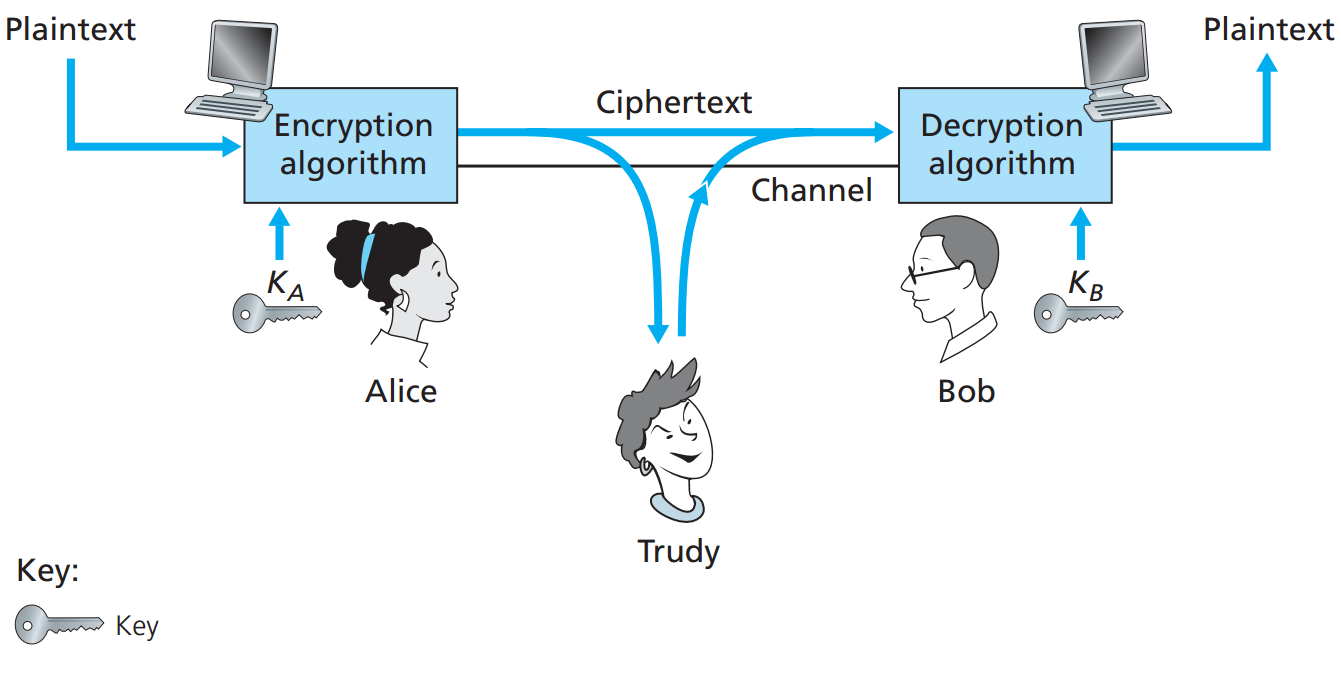
\includegraphics[width=14cm]{img/basic_crypto}}
  \centering
  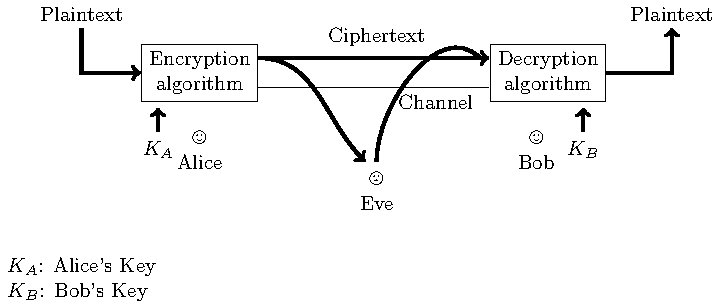
\includegraphics[width=\textwidth]{../img/basiccryptosystem}
  \caption[Basic cryptosystem diagram]{Basic cryptosystem diagram. Based on Kurose and Ross \cite{kurose2010computer}.}
  \label{fig:cryptoflow}
\end{figure}


\end{frame}

%------------------------------------------------
%\subsection{Abstract Algebra}
\begin{frame}
\frametitle{Abstract Algebra}

Abstract algebra is a branch of mathematics that focuses on those elements that can be operated algebraically. Groups and rings are examples of such sets of elements \cite{CryptoStallings}. \\~\\
\begin{block}{Definition of Group}
A \emph{group} G, denoted by $\{ G, \cdot \}$ is a set of elements with a binary operation, which is denoted by the operator $\cdot$.
\end{block}

\begin{block}{Definition of Ring}
A \emph{ring} $R$, which is sometimes denoted by $\{R, +, \times \}$, is a set of elements with two binary operations, called \textit{addition} and \textit{multiplication}, such that for all $a$, $b$, $c$ in $R$, there are some axioms that must be obeyed.
\end{block}

\end{frame}

%------------------------------------------------

\begin{frame}
\frametitle{Homomorphisms}

A \emph{homomorphism} consists of the construction of a function that \emph{translates} elements from one group to another group with the same properties.

\begin{block}{Definition}
Let $G_{1}$ and $G_{2}$ be groups, and let $\phi: G_{1} \rightarrow G_{2}$ be a function. Then $\phi$ is said to be a \textbf{group homomorphism} if
\begin{equation}
\phi(a*b) = \phi(a) *' \phi(b)
\end{equation}
for all $a$, $b$ in $G_{1}$.
\end{block}

In the case for rings, a homomorphism considers two operations instead.

\end{frame}
%------------------------------------------------
\begin{frame}
\frametitle{Jewelry Store Analogy}

\begin{enumerate}
  \setlength\itemsep{1.5em}
\item Alice has a jewelry store and wants her workers to assemble raw materials into finished products.
\item Alice places the materials inside transparent glove boxes, which are then locked with her key.
\item Workers can put their hands inside the gloves that are connected to the box to work with the raw materials. 
\item The workers are able to put in things inside the boxes, i.e.\ soldering iron. 
\item Once the products are finished, Alice can then recover the products from the box using her key. 
\end{enumerate}

\end{frame}

%------------------------------------------------

%\subsection{Homomorphic Encryption}
\begin{frame}
\frametitle{Homomorphic Encryption}
\begin{itemize}
\item Refers to the ability to perform computations on encrypted data without sharing the secret key to decrypt the data prior to the computations. \\~\\
\item When the encryption function of a cryptosystem is a homomorphism, meaning that it preserves group operations performed on ciphertexts, it is called a \emph{homomorphic cryptosystem}. \\~\\
\item Lange \cite{lange2011} mentions that several real life applications of homomorphic encryption fall in the domain of: e-cash, e-voting, private information retrieval, and cloud computing.
\end{itemize}
\end{frame}

%------------------------------------------------
\begin{frame}
\frametitle{Additive and Multiplicative Homomorphic Encryption}

A homomorphic encryption is additive if:
\begin{equation}
\mathcal{E}(x+y) = \mathcal{E}(x)\otimes \mathcal{E}(y),
\end{equation}
where $\mathcal{E}$ denotes an encryption function, $\otimes$ denotes an operation depending on the used cipher and $x$ and $y$ are plaintext messages. \\~\\

A homomorphic encryption is multiplicative if:
\begin{equation}
\mathcal{E}(x \cdot y) = \mathcal{E}(x) \otimes \mathcal{E}(y),
\end{equation}
where again $\mathcal{E}$ denotes an encryption function, $\otimes$ denotes an operation depending on the used cipher and $x$ and $y$ are plaintext messages.

\end{frame}

%------------------------------------------------
\begin{frame}
\frametitle{Classification of Homomorphic Encryption Schemes}
\begin{itemize}
  \setlength\itemsep{1.5em}
\item \emph{Partially homomorphic encryption} schemes are defined over a group, and they support one operation at most: either addition or multiplication.  
\item \emph{Fully homomorphic encryption} schemes are defined over a ring, and can support up to two operations: addition and multiplication. 
\item \emph{Somewhat homomorphic encryption} schemes support up to two operations; however, the number of operations that can be performed is limited.
\end{itemize}

\end{frame}
%------------------------------------------------
%\subsection{Services in the Cloud}
\begin{frame}
\frametitle{Services in the Cloud}
The cloud, a trendy term used to describe a network of servers usually accessible through the Internet, currently provides two important services: storage and computation. \\~\\

One of the main advantages of employing a service in the cloud is that the owners are relieved from the burden of data storage and maintenance at all times. \\~\\

By relying on a cloud service, the owner is relieved of the control and protection of the data, raising security concerns. \\~\\

Attempts to tackle these concerns include \emph{secure multi-party computation} and \emph{homomorphic encryption}. 
\end{frame}
%------------------------------------------------
\section{Methodology}
%\subsection{Case Study}
\begin{frame}
\frametitle{Case Study}

\begin{itemize}
  \setlength\itemsep{1.5em}
\item Consider a household that has a pattern of activity, fluctuating during the day.
\item The resident seeks to ascertain the number of people inside at any point in time.
\item Assume the resident has put in place certain sensors around the building to detect entry and exit.
\item Counter of people inside is stored in the cloud for subsequent retrieval. 
\item Resident does not want others to learn of this value, as to prevent potential burglars to break in when the household is empty.
\end{itemize}
\end{frame}

%------------------------------------------------

%\subsection{Proposed Solution}
\begin{frame}
\frametitle{Proposed Solution}

Implementation of a client-server software that aims to store and modify securely a counter by making use of homomorphic encryption.  \\~\\~\\

The solution utilizes a \emph{HElib}, a library in C++ that enables the use of a leveled fully homomorphic encryption scheme. It is used to perform operations on the encrypted data, such as addition, subtraction, and multiplication. \\~\\

\end{frame}

%------------------------------------------------
\begin{frame}
\frametitle{Architecture Breakdown}
\begin{figure}[H]
  \centering
  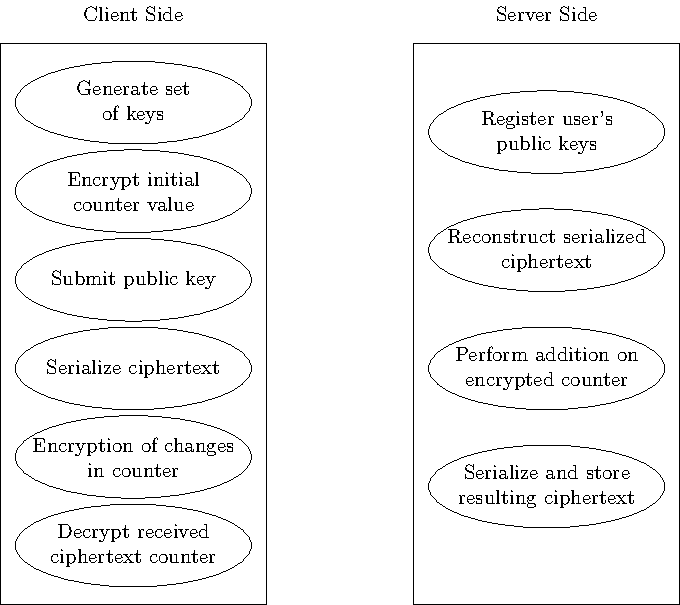
\includegraphics[scale=0.65]{../img/architecture}
 \caption{Architecture breakdown into client and server.}
 \label{fig:clientserver}
\end{figure}

\end{frame}
%------------------------------------------------
\begin{frame}
\frametitle{Operation Flow}
\begin{enumerate}
	\item Parameters to use with the HElib are arbitrarily chosen or calculated.
	\item Public and private keys are created.
	\item The public key is serialized and sent to the server.
	\item The structures to store plaintext and ciphertext are declared.
	\item The initial counter value is set into the plaintext structure.
	\item The plaintext is encrypted using the public key and stored into the ciphertext structure.
        \item The encrypted counter is sent to the server.
	\item Values are added or substracted from the ciphertext.
	\item Ciphertext is decrypted using the private key, and its value is stored in another plaintext structure.
\end{enumerate}
\end{frame}

%------------------------------------------------
\begin{frame}
\frametitle{Sequence Diagram}

\begin{figure}[H]
  \centering
  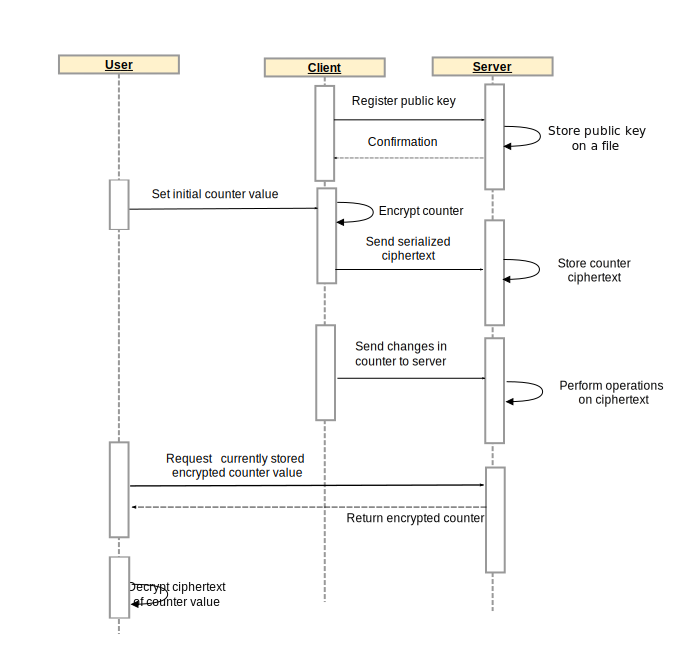
\includegraphics[scale=0.35]{../img/counter}
  \caption{Sequence diagram showing operation under normal conditions}
  \label{fig:seqdiag}
\end{figure}
\end{frame}

%------------------------------------------------
\begin{frame}
\frametitle{Implementation Details}
\begin{itemize}
  \setlength\itemsep{1.5em}
\item A seed is used to pseudorandomly generate the set of keys.
\item Among the parameters chosen, the security parameter $k$ is chosen at the start.
\item Serialization is done by using the \emph{istringstream} and \emph{ostringstream} C++ classes.
\item Communication between client and server is done by using sockets on TCP.
\end{itemize}
\end{frame}

%------------------------------------------------
\section{Experiments and Results}
%\subsection{Setup}
\begin{frame}
\frametitle{Setup}
The experiment is performed by running several iterations of the program with different values of the security parameter $k$. The experimental units considered where: 
\begin{itemize}
\item \textbf{Times for}: key generation, encryption, decryption, and homomorphic addition of ciphertext. 
\item \textbf{Sizes for}: public key and ciphertext.
\end{itemize}

\vspace*{5mm} 
The experiment considers several arbitrarily chosen values, namely: 20, 40, 80, 100; where 80 is the default value found in the examples of the HElib.

\begin{itemize}
\item Iterations were run on a notebook which had an AMD Elite A4-5150M processor. 
\item The processor is dual core and it runs at 2.7 GHz. 
\end{itemize}
\end{frame}
%------------------------------------------------
%\subsection{Results}
\begin{frame}
\frametitle{Results}

\begin{table}[h]
  \caption{Experimental results}
  \label{tbl:results}
\resizebox{\columnwidth}{!}{%
\begin{tabular}{lrrrrrr}
\toprule
\textbf{k}   & \textbf{Key Gen.} & \textbf{Key Size}  & \textbf{Encryption} & \textbf{Decryption} & \textbf{Addition} & \textbf{Ctext Size} \\
\midrule
40  & 13.130 s & 165.922 MB & 0.355 s    & 0.048 s    & 0.074 s  & 30.977 kB        \\
60  & 10.710 s & 91.635 MB  & 0.414 s    & 0.056 s    & 0.077 s  & 36.053 kB        \\
80  & 8.380 s  & 57.080 MB  & 0.642 s    & 0.057 s    & 0.082 s  & 37.745 kB        \\
100 & 9.529 s  & 35.453 MB  & 0.579 s    & 0.064 s    & 0.082 s  & 43.676 kB
\end{tabular}%
}
\end{table}

\end{frame}
%------------------------------------------------
\begin{frame}
\frametitle{Results: Key Generation}
Figure \ref{fig:boxplot} depicts a box plot that shows the time required to generate the set of keys depending on the size of $k$.
\vspace*{-5mm} 
\begin{figure}[h]
  \centerline{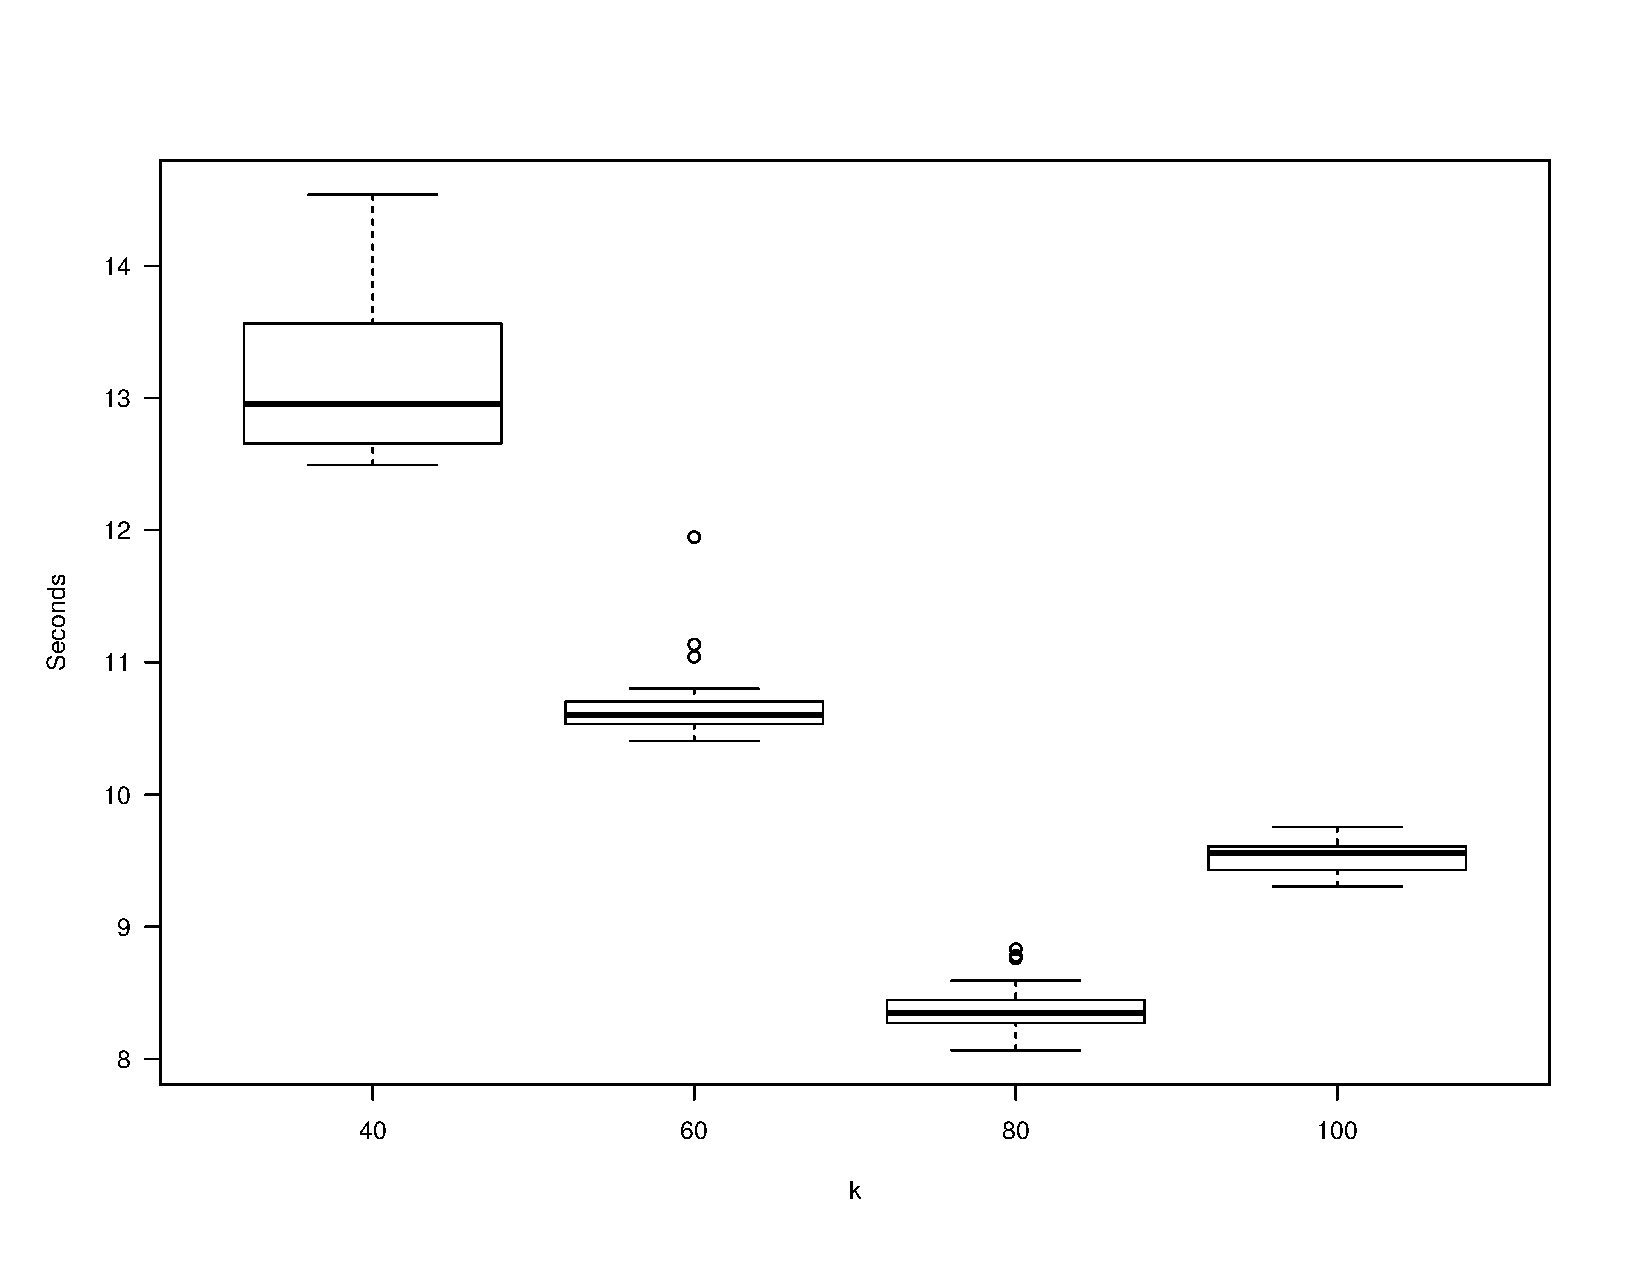
\includegraphics[height=6cm]{../img/experimentplot}}
  \vspace*{-5mm} 
  \caption{Key generation time}
  \label{fig:boxplot}
\end{figure}


\end{frame}
%------------------------------------------------
\section{Related Works}
\begin{frame}
\frametitle{Related Works}

\begin{table}[]
\centering
\caption{Comparison between related works}
\label{tbl:comparison}
\resizebox{\columnwidth}{!}{%
\begin{tabular}{|l|c|c|c|c|c|c|c|}
\hline
\multicolumn{1}{|c|}{Characteristic / Work}                                   & \multicolumn{1}{l|}{\begin{tabular}[c]{@{}l@{}}Yasuda \\ et al.\ \cite{Yasuda:2015:SDD:2732516.2732521}\end{tabular}} & \multicolumn{1}{l|}{\begin{tabular}[c]{@{}l@{}}Yasuda \\ et al.\ \cite{yasuda2014}\end{tabular}} & \multicolumn{1}{l|}{\begin{tabular}[c]{@{}l@{}}Adida \\ et al.\ \cite{adida2008helios}\end{tabular}} & \multicolumn{1}{l|}{Cybernetica \cite{ESORICS08:BLW08}} & \multicolumn{1}{l|}{\begin{tabular}[c]{@{}l@{}}Tetali \\ et al.\ \cite{Tetali:2013:MSA:2544173.2509554}\end{tabular}} & \multicolumn{1}{l|}{\begin{tabular}[c]{@{}l@{}}Schroepfer\\  et al.\ \cite{Schroepfer:2011:DSC:2046707.2093509}\end{tabular}} & \multicolumn{1}{l|}{Thesis work} \\ \hline
Client-server architecture                                                    & $\times$                                                                             & $\times$                                                                             & $\checkmark$                                                                            & $\sim$                               & $\checkmark$                                                                             & $\times$                                                                                 & $\checkmark$                                \\ \hline
Cloud computation                                                             & $\checkmark$                                                                             & $\times$                                                                             & $\checkmark$                                                                            & $\checkmark$                                & $\checkmark$                                                                             & $\times$                                                                                 & $\checkmark$                                \\ \hline
Real-world application                                                        & $\checkmark$                                                                             & $\times$                                                                             & $\checkmark$                                                                            & $\checkmark$                                & $\times$                                                                             & $\checkmark$                                                                                 & $\checkmark$                                \\ \hline
Secure computation                                                            & $\checkmark$                                                                             & $\checkmark$                                                                             & $\checkmark$                                                                            & $\checkmark$                                & $\checkmark$                                                                             & $\checkmark$                                                                                 & $\checkmark$                                \\ \hline
\begin{tabular}[c]{@{}l@{}}Homomorphic addition \\ support\end{tabular}       & $\checkmark$                                                                             & $\times$                                                                             & $\checkmark$                                                                            & $\times$                                & $\times$                                                                             & $\times$                                                                                 & $\checkmark$                                \\ \hline
\begin{tabular}[c]{@{}l@{}}Homomorphic multiplication \\ support\end{tabular} & $\checkmark$                                                                             & $\times$                                                                             & $\times$                                                                            & $\times$                                & $\times$                                                                             & $\times$                                                                                 & $\checkmark$                                \\ \hline
No 3rd party trust                                                       & $\times$                                                                             & $\checkmark$                                                                             & $\checkmark$                                                                            & $\checkmark$                                & $\checkmark$                                                                             & $\times$                                                                                 & $\checkmark$                                \\ \hline
Key exchange support                                                          & $\checkmark$                                                                             & $\checkmark$                                                                             & $\checkmark$                                                                            & $\times$                                & $\times$                                                                             & $\checkmark$                                                                                 & $\times$                                \\ \hline
Web-based                                                                     & $\times$                                                                             & $\times$                                                                             & $\checkmark$                                                                            & $\checkmark$                                & $\times$                                                                             & $\checkmark$                                                                                 & $\times$                                \\ \hline
\end{tabular}%
}
\end{table}
\vspace*{-5mm} 

\begin{table}[]
\centering
\resizebox{\columnwidth}{!}{%
\begin{tabular}{|l|l|l|}
\hline
{\it $\checkmark$ has the characteristic} & {\it $\sim$ partially has the characteristic} & {\it $\times$ does not have the characteristic} \\ \hline
\end{tabular}%
}
\end{table}
\end{frame}
%------------------------------------------------------------

\section{Conclusions}
\begin{frame}
\frametitle{Conclusions}

In essense, a client-server archictecture was established and it made use of homomorphic encryption successfully. \\~\\

Factors that pose a challenge for implementation: key generation time, key size, ciphertext size, and encryption and decryption times. \\~\\

It was chosen to experiment on the value of the security parameter $k$. Data regarding the execution times and size of the key and ciphertext were collected. \\~\\

The results showed that key generation ranged between 9 and 13 seconds, while the size of the public key ranged between 35 and 165 megabytes.
\end{frame}
%------------------------------------------------
\begin{frame}
\frametitle{Contributions}
\begin{itemize}
  \setlength\itemsep{1.5em}
\item Design and implementation of a client-server architecture based software that employs homomorphic encryption was made.
\item A case study was addressed, closing the gap between the theory of homomorphic encryption and actual practice.
\item Data regarding the use of the functionalities provided by HElib was gathered.
\end{itemize}
\end{frame}
%------------------------------------------------
\begin{frame}
\frametitle{Future Work}
\begin{itemize}
\item Design and implement the appropriate mechanisms for key management.
\item Design a database scheme to keep track of the ciphertexts stored in the server.
\item Look into the possibility of implementing the client-architecture system as a Software-as-a-Service model.
\item Provide a secure communication channel between the client and server, relying on the SSL/TLS protocol.
\item Experiment on the number of homomorphic operations correctly evaluated before the accumulated noise causes an incorrect decryption.
\item Implement solution over the HTTPS protocol, as to allow its use via web browsers.
\end{itemize}

\end{frame}

%------------------------------------------------

\begin{frame}[allowframebreaks]{References}
%\frametitle{References}
\def\newblock{}
\bibliographystyle{abbrv}
\bibliography{bibliografia}
\end{frame}

%------------------------------------------------

\end{document} 
